% !TeX root = main.tex

\hypertarget{approximating-area}{%
\section{Approximating Area}\label{approximating-area}}

\hypertarget{what-is-an-area-and-how-to-measure-it}{%
\subsection{What is an area and how to measure
it}\label{what-is-an-area-and-how-to-measure-it}}

The area of a shape can be measured by comparing the shape to squares of
a fixed size, say \(1\times1\) sized square. For a regular shape such as
a rectangle, the area can be easily measured by dividing the rectangle
into squares and taking the sum. This simple idea can be generalized to
measure irregular areas approximately. The accurate measurement of an
irregular shape needs the limit.

For areas under curve \(f\), we take the following approach.

\begin{enumerate}[sepno]
\item
  Dividing the interval \([a,b]\) into n subintervals of equal width,
  \(\Delta x=\dfrac{b - a}{n}\). Let \(x_0,x_1,x_2, \dots ,x_n\) with
  \(x_0=a,x_n=b,\) and \(x_i=x_0+i\Delta x\) be the boundary points of
  those subintervals.
\item
  The area under the curve over a subinterval \([x_{i-1}, x_i]\) can by
  estimated by \(f(x_i^*)\Delta x\), where \(x_i^*\) is a point in the
  interval \([x_{i-1}, x_i]\), and \(i=1,2,\dots, n\).
\item
  The area under the curve over \([a, b]\) is then approximately
  \[ f(x_1^*)\Delta x+f(x_2^*)+\cdots +f(x_{n-1}^*)\Delta x+f(x_n^*)\Delta x.\]
\end{enumerate}

% 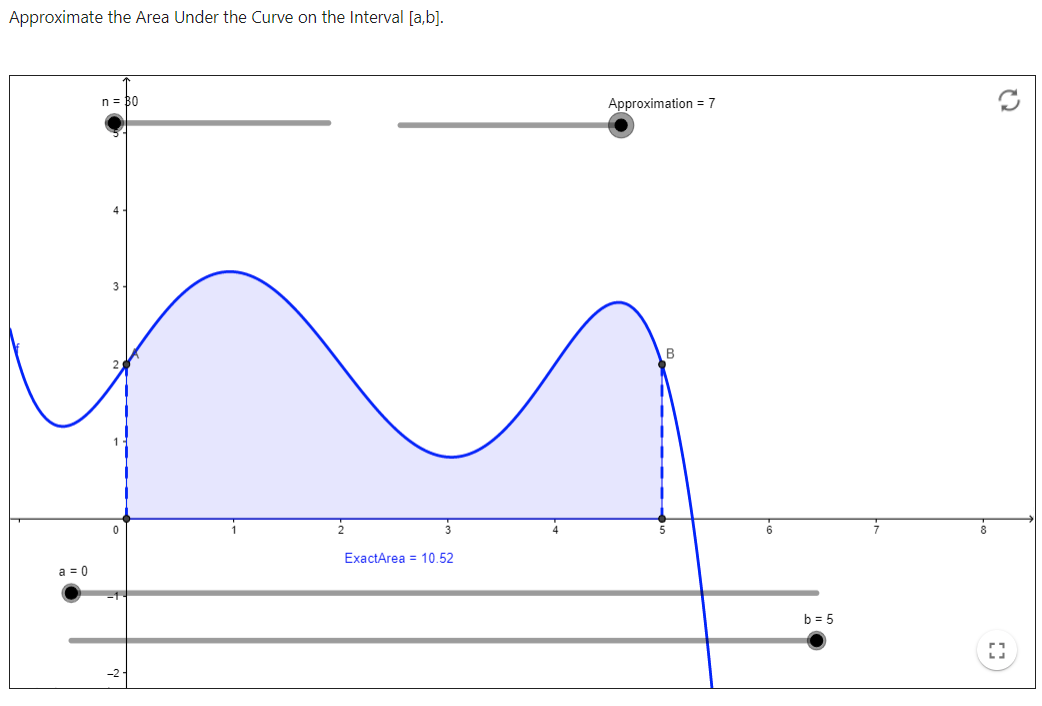
\includegraphics[width=0.9\textwidth]{img/image-20200422234011771.png}


\hypertarget{sigma-notation}{%
\subsection{Sigma Notation}\label{sigma-notation}}

For convenience, we use sigma notation \(\sum\limits_{i=1}^n s_n\) to
write sums of a sequence of \(n\) values \(s_1\),\(s_2\),\(\dots\),
\(s_n\). In the sigma notation, the letter \(i\) is called \textbf{the
index}, \(1\) is the starting value and \(n\) is the ending value in the
sequence.

For example,

\[\sum\limits_{i=1}^nf(x_i^*)\Delta x:=f(x_1^*)\Delta x+f(x_2^*)+\cdots +f(x_{n-1}^*)\Delta x+f(x_n^*)\Delta x.\]

\[\sum\limits_{n=1}^{100}n:=1+2+3+\cdots+100.\]

\hypertarget{properties-of-sigma-notation}{%
\subsection{Properties of Sigma
Notation}\label{properties-of-sigma-notation}}

Let \(a_1,a_2, \dots ,a_n\) and \(b_1,b_2, \dots ,b_n\) represent two sequences of
terms and let \(c\) be a constant. The following properties hold for all
positive integers \(n\) and for integers \(m\), with \(1 \le m \le n.\)

\begin{enumerate}[sepno]
\item
  \(\displaystyle \sum_{i=1}^n c=nc\)
\item
  \(\displaystyle \sum_{i=1}^n ca_i=c\sum_{i=1}^na_i\)
\item
  \(\displaystyle \sum_{i=1}^n(a_i+b_i)=\sum_{i=1}^na_i+\sum_{i=1}^nb_i\)
\item
  \(\displaystyle \sum_{i=1}^n(a_i - b_i)=\sum_{i=1}^na_i - \sum_{i=1}^nb_i\)
\item
  \(\displaystyle \sum_{i=1}^na_i=\sum_{i=1}^ma_i+\sum_{i=m+1}^na_i\)
\end{enumerate}

\hypertarget{sum-of-powers-of-a-sequence-of-integers}{%
\subsection{Sum of powers of a sequence of
integers}\label{sum-of-powers-of-a-sequence-of-integers}}

\[\sum_{i=1}^n i=1+2+ \cdots +n=\dfrac{n(n+1)}{2}\]

\[\sum_{i=1}^n i^2=1^2+2^2+ \cdots +n^2=\dfrac{n(n+1)(2n+1)}{6}\]

\[\sum_{i=1}^n i^3=1^3+2^3+ \cdots +n^3=\dfrac{n^2(n+1)^2}{4} \]

\begin{example}

Find the sum of the values of \(2n-1\) for \(n=1,2, \dots ,100\).

\end{example}
\vspace*{6\baselineskip}

\begin{example}

Find the sum of the values of \(n^2-n+1\) for \(n=1,2, \dots ,100\).

\end{example}
\vspace*{6\baselineskip}

\hypertarget{approximating-areas}{%
\subsection{Approximating Areas}\label{approximating-areas}}

\begin{definition}

A set of points \(P={x_i}\) for \(i=0,1,2, \dots ,n\) with
\(a=x_0<x_1<x_2< \cdots <x_n=b\), which divides the interval \([a,b]\) into
subintervals of the form
\([x_0,x_1]\),\([x_1,x_2]\),\ldots,\([x_{n - 1},x_n]\) is called a
\textbf{partition} of \([a,b]\). If the subintervals all have the same
width, the set of points forms a \textbf{regular partition} of the
interval \([a,b]\).

\end{definition}

\begin{definition}

Let \(f\) be a continuous function. The sum
\[L_n=\sum\limits_{i=1}^nf(x_{i - 1})\Delta x=f(x_0)\Delta x+f(x_1)\Delta x+\cdots+f(x_{n - 1})\Delta x,\]
where \(x_0=a\), \(\Delta=\frac{b-a}{n}\) and \(x_i=a+(i-1)\Delta x\),
is called a \textbf{left-endpoint approximation} of the area under \(f\)
over the interval \([a,b]\).

Let \(f\) be a continuous function. The sum
\[R_n=\sum\limits_{i=1}^nf(x_{i})\Delta x=f(x_1)\Delta x+f(x_1)\Delta x+\cdots+f(x_{n})\Delta x,\]
where \(x_0=a\), \(\Delta=\frac{b-a}{n}\) and \(x_i=a+(i-1)\Delta x\),
is called a \textbf{right-endpoint approximation} of the area under
\(f\) over the interval \([a,b]\).

\href{https://www.geogebra.org/m/kajgu9Yu}{Definite Integral Approximations by jeromeawhite}
% {\centering 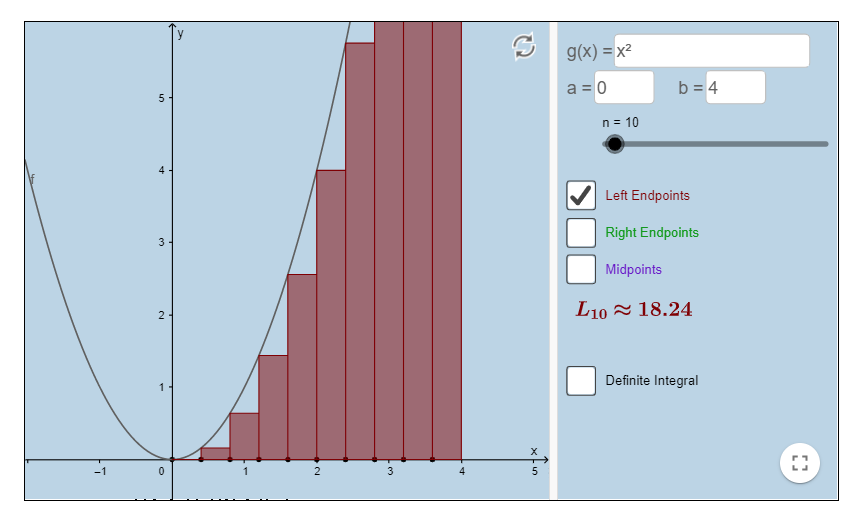
\includegraphics[scale=0.3]{img/image-20200422234746363.png}}

\end{definition}

\begin{example}

Find the left-endpoint and right-endpoint approximation of the area
under the curve \(f(x)=x^2\) over the interval \([0, 2]\) using a
partition of \(n=10\) subintervals.

\end{example}
\vspace*{6\baselineskip}

\hypertarget{riemann-sum}{%
\subsection{Riemann Sum}\label{riemann-sum}}

\begin{definition}

Let \(f(x)\) be defined on a closed interval \([a,b]\) and let \(P\) be
a regular partition of \([a,b]\). Let \(\Delta x\) be the width of each
subinterval \([x_{i - 1},x_i]\) and for each \(i\), let \(x^*_i\) be any
point in \([x_{i - 1},x_i]\). A \textbf{Riemann sum} is defined for
\(f(x)\) as \[RM_n:=\sum\limits_{i=1}^nf(x^*_i)\,\Delta x.\]

\end{definition}

\begin{definition}

A function is integrable if \(\lim\limits_{n\to \infty}R_n=A\) for any
partition of \([a, b]\).

\end{definition}

\textbf{Fact:} All functions which are continuous except at finitely
many removable or jumping discontinuities are integral.

A proof of this fact uses the \textbf{upper sum} and \textbf{lower sum}
where the sample points are where the function has max and min value
respectively. in the subinterval. Because of the continuity, the
difference between the maximum value and minimum value of \(f\) can be
make arbitrarily small by restricting to sufficiently small intervals.
That will make the difference between the upper and lower Riemann sums
neglectable.

% 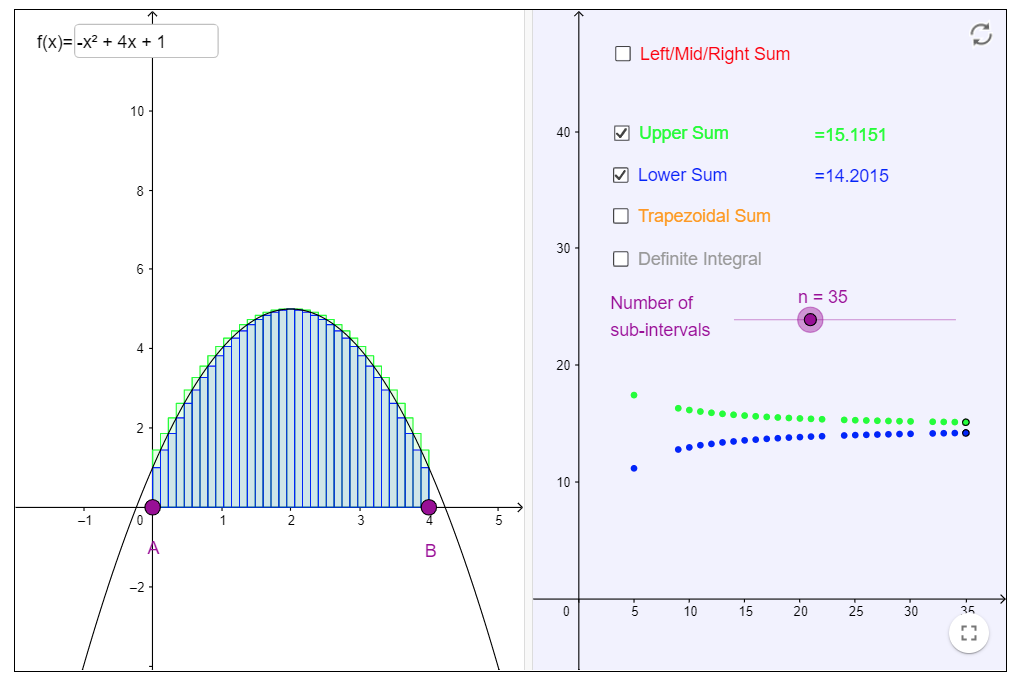
\includegraphics[width=0.9\textwidth]{img/image-20200422234550315.png}

\textbf{Fact:} For an integrable function \(f\), the area under the
curve \(f\) over \([a, b]\) is the limit of any Riemann sum. The
midpoint is also frequently used to calculate the Riemann sum.

\begin{example}

Find the lower sum and the upper sum for \(f(x)=1 - x^2\) on \([1,2]\)
using a regular partition of \(n=4\) subintervals.

\end{example}
\vspace*{6\baselineskip}

% \hypertarget{definite-integral}{%
% \subsection{Definite Integral}\label{definite-integral}}

% Let \(f(x)\) be an integrable function, particularly, a continuous
% function, defined over an interval \([a,b]\). The \textbf{definite
% integral} of \(f\) from \(a\) to \(b\) is defined as
% \[\int^b_af(x)\mathrm{d}x=\lim\limits_{n\to\infty}\sum\limits_{i=1}^nf(x^*_i)\Delta x.\]
% The numbers \(a\) and \(b\) are called the upper and lower limits of
% integration. The function \(f(x)\) is called the integrand. The
% differential \(\mathrm{d} x\) is called the variable of integration.

% Like the index in a sigma notation, the variable of integration is a
% dummy variable, which mean you may use any other letter instead of \(x\)
% to write the integral.

% \textbf{Fact:} The definite integral \(\int_a^bf(x)\mathrm{d}x\) is the
% signed area under the curve \(f\) over the interval \([a, b]\).

% \begin{example}

% Find the definite integral \(\int_0^2x\mathrm{d}x\) using a Riemann sum
% and a graph.

% \end{example}
% \vspace*{6\baselineskip}

% \begin{example}

% Find the definite integral \(\int_0^1\sqrt{1-x^2}\mathrm{d}x\) using a
% graph.

% \end{example}
% \vspace*{6\baselineskip}

\subsection{Practice}

\begin{exercise}

Find the sum of the values of \(3n+2\) for \(n=1,2, \dots ,100\).

\end{exercise}
\vspace*{6\baselineskip}

\begin{exercise}

Find the lower sum and the upper sum for \(f(x)=x^2-2x\) on \([0,2]\)
using a regular partition of \(n=5\) subintervals.

\end{exercise}
\vspace*{6\baselineskip}

% \begin{exercise}

% Find the definite integral \(\int_0^2(2x+1)\mathrm{d}x\) using a Riemann
% sum and a graph.

% \end{exercise}
% \vspace*{6\baselineskip}

% \begin{exercise}

% Find the definite integral \(\int_{-2}^0\sqrt{4-x^2}\mathrm{d}x\) using
% a graph.

% \end{exercise}

